% Generated by scripts/generate_article_concordance_country_outputs.py. Do not edit.
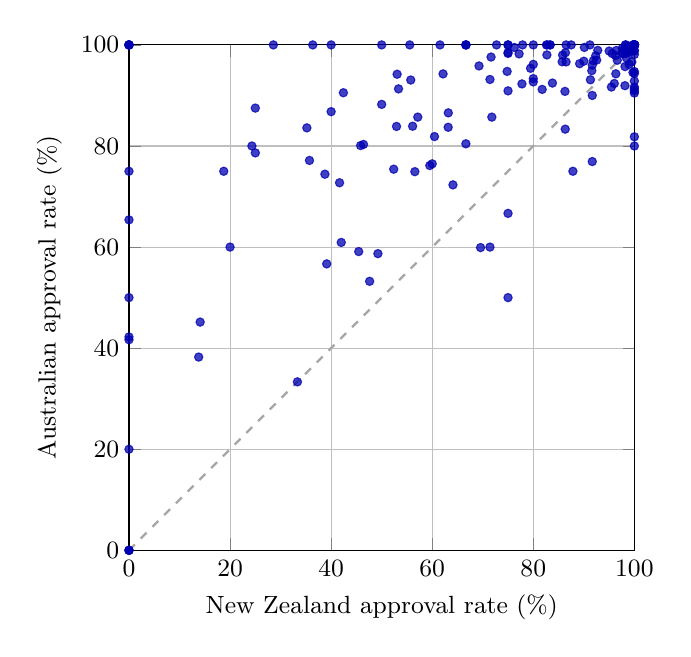
\begin{tikzpicture}
\begin{axis}[
  width=0.78\textwidth, height=8.0cm,
  xmin=0, xmax=100, ymin=0, ymax=100,
  xlabel={New Zealand approval rate (\%)}, ylabel={Australian approval rate (\%)},
  axis equal image, grid=major, tick label style={font=\small}, label style={font=\small},
]
\addplot[gray!70, dashed, thick, domain=0:100] {x};
\addplot[only marks, mark=*, mark size=1.5pt, blue!70!black, opacity=0.75] coordinates {(14.08450704,45.16129032) (71.42857143,60) (41.66666667,72.72727273) (0,100) (85.80060423,98) (50,88.23529412) (100,98.91304348) (80,92.68292683) (100,100) (100,94.73684211) (55.75176589,93.05662222) (100,100) (75,90.90909091) (99.46236559,98.71794872) (100,100) (28.57142857,100) (50,100) (63.17991632,86.55883286) (82.60869565,100) (100,100) (75,98.31460674) (89.17041275,96.28482972) (100,100) (83.33333333,100) (0,65.38461538) (100,100) (91.57212318,94.90899499) (13.79310345,38.23529412) (98.57142857,99.29938022) (0,75) (90.10380623,99.5049505) (96.62268832,96.96474355) (98.13886901,98.47165992) (92.75362319,98.92473118) (74.82337829,94.75703325) (0,0) (87.5,100) (100,80) (98.96907216,96.15384615) (0,100) (18.75,75) (99.6875,100) (0,100) (66.66666667,100) (61.53846154,100) (71.42857143,93.16239316) (56.12244898,83.91608392) (100,92.85714286) (75,66.66666667) (100,90.90909091) (80,100) (64.1025641,72.30769231) (79.45879459,95.37480064) (91.20879121,100) (97.75390625,98.24742268) (57.14285714,85.71428571) (99.61389961,99.47589099) (45.45454545,59.11111111) (91.66666667,96) (75,100) (75,98.48484848) (0,100) (83.33333333,100) (20,60) (72.72727273,100) (98.21428571,100) (100,100) (56.56214891,74.92176595) (95.0105042,98.78644868) (53.05466238,94.19942474) (47.61904762,53.22580645) (98.13084112,91.93548387) (86.48648649,100) (99.49937422,96.6442953) (91.66666667,90) (99.56498814,99.61618981) (59.52380952,76.13293051) (76.25,99.48979592) (46.4028777,80.30969397) (77.88461538,100) (98.40848806,98.33119384) (66.66666667,80.43478261) (96.02649007,92.36947791) (91.66666667,76.92307692) (69.56521739,59.89761092) (0,41.66666667) (36.36363636,100) (100,100) (90,96.77419355) (100,91.66666667) (0,50) (60,76.47058824) (97.57820383,98.47992196) (82.69230769,98.01980198) (75,50) (100,81.81818182) (100,100) (86.48648649,96.6396292) (92.34042553,97.84313725) (100,100) (60.4519774,81.86813187) (52.94117647,83.87096774) (80,96.15384615) (49.25606891,58.7012987) (55.55555556,100) (100,100) (38.76935727,74.42020567) (98.98989899,99.36305732) (100,100) (0,100) (42,60.91891892) (100,94.36619718) (98.30097087,99.54493743) (95.62043796,98.28767123) (39.12419239,56.6753136) (91.89189189,96.875) (86.26760563,90.80267559) (86.36363636,98.46153846) (71.64179104,97.6) (83.78879111,92.45380407) (100,98.80952381) (96.2962963,97.89029536) (98.47130762,99.00405132) (91.30434783,93.10344828) (69.26286509,95.83952452) (52.38095238,75.40983607) (66.66666667,100) (100,100) (95.45454545,91.66666667) (77.19298246,98.22298653) (0,0) (75,100) (100,90.47619048) (0,42.22222222) (96.43705463,98.89843845) (100,91.30434783) (100,100) (96.33027523,94.28571429) (0,20) (62.14511041,94.26751592) (33.33333333,33.33333333) (99.72222222,94.55445545) (77.7544596,92.28429337) (53.33333333,91.30434783) (35.71428571,77.14285714) (100,100) (98.75,99.71014493) (98.04347826,99.36708861) (24.32432432,80) (97.62340037,99.3460678) (66.66666667,100) (92.54165052,96.99547993) (98.14814815,95.71428571) (0,0) (86.31578947,83.33333333) (80,93.33333333) (40,100) (98.30508475,100) (35.2,83.58585859) (45.83333333,80.08752735) (85.71428571,96.66666667) (100,98.10901001) (98.41954023,97.42366412) (42.42424242,90.54054054) (98.35632521,98.65906805) (82.75862069,100) (25,78.6389414) (87.83783784,75) (71.79487179,85.71428571) (81.75313059,91.19648318) (25,87.5) (63.15789474,83.7037037) (40,86.79504814)};
\end{axis}
\end{tikzpicture}
